\documentclass[12pt,a4paper,openany,oneside]{book}


% 格式控制
%------------------------------------------------------------------------------%
%                                                                              %
%   LaTeX Template for Bachlor Thesis of Northwestern Polytechnical University %
%   Environment Config: TeXLive 2017                                           %
%   * XeTeX 3.14159265-2.6-0.99998 (TeX Live 2017/W32TeX)                      %
%   * BibTeX 0.99d (TeX Live 2017/W32TeX)                                      %
%   Version: 1.5.0.0426                                                        %
%                                                                              %
%------------------------------------------------------------------------------%
%   Copyright by NWPU Metaphysics Office, GPLv3-LICENSE                        %
%------------------------------------------------------------------------------%


%---------------------------------纸张大小设置---------------------------------%
\usepackage{geometry}
% 普通A4格式缩进
% \geometry{left=2.5cm,right=2.5cm,top=2.5cm,bottom=2.5cm}
% 论文标准缩进
\geometry{left=1.25in,right=1.25in,top=1in,bottom=1.5in}
%------------------------------------------------------------------------------%


%----------------------------------必要库支持----------------------------------%
\usepackage{xcolor}
\usepackage{tikz}
\usepackage{layouts}
\usepackage[numbers,sort&compress]{natbib}
\usepackage{clrscode}
\usepackage{gensymb}
\usepackage[final]{pdfpages}
\usepackage{algorithm, algorithmicx, algpseudocode}
\renewcommand{\algorithmicrequire}{\textbf{Input:}}
\renewcommand{\algorithmicensure}{\textbf{Output:}} 
%------------------------------------------------------------------------------%


%--------------------------------设置标题与目录--------------------------------%
\usepackage[sf]{titlesec}
\usepackage{titletoc}
%------------------------------------------------------------------------------%


%--------------------------------添加书签超链接--------------------------------%
\usepackage[unicode=true,colorlinks=false,pdfborder={0 0 0}]{hyperref}
% 在此处修改打开文件操作
\hypersetup{
    bookmarks=true,         % show bookmarks bar?
    pdftoolbar=true,        % show Acrobat’s toolbar?
    pdfmenubar=true,        % show Acrobat’s menu?
    pdffitwindow=true,      % window fit to page when opened
    pdfstartview={FitH},    % fits the width of the page to the window
    pdfnewwindow=true,      % links in new PDF window
}
% 在此处添加文章基础信息
\hypersetup{
    pdftitle={title},
    pdfauthor={author},
    pdfsubject={subject},
    pdfcreator={creator},
    pdfproducer={producer},
    pdfkeywords={key1  key2  key3}
}
%------------------------------------------------------------------------------%


%---------------------------------设置字体大小---------------------------------%
\usepackage{type1cm}
% 字号与行距,统一前缀s(a.k.a size)
\newcommand{\sChuhao}{\fontsize{42pt}{63pt}\selectfont}                 % 初号, 1.5倍
\newcommand{\sYihao}{\fontsize{26pt}{36pt}\selectfont}                  % 一号, 1.4倍
\newcommand{\sErhao}{\fontsize{22pt}{28pt}\selectfont}                  % 二号, 1.25倍
\newcommand{\sXiaoer}{\fontsize{18pt}{18pt}\selectfont}                 % 小二, 单倍
\newcommand{\sSanhao}{\fontsize{16pt}{24pt}\selectfont}                 % 三号, 1.5倍
\newcommand{\sXiaosan}{\fontsize{15pt}{22pt}\selectfont}                % 小三, 1.5倍
\newcommand{\sSihao}{\fontsize{14pt}{21pt}\selectfont}                  % 四号, 1.5倍
\newcommand{\sHalfXiaosi}{\fontsize{12.5pt}{16.25pt}\selectfont}        % 半小四, 1.25倍
\newcommand{\sLargeHalfXiaosi}{\fontsize{13pt}{19pt}\selectfont}        % 半小四, 1.5倍
\newcommand{\sXiaosi}{\fontsize{12pt}{14.4pt}\selectfont}               % 小四, 1.25倍
\newcommand{\sLargeWuhao}{\fontsize{11pt}{11pt}\selectfont}             % 大五, 单倍
\newcommand{\sWuhao}{\fontsize{10.5pt}{10.5pt}\selectfont}              % 五号, 单倍
\newcommand{\sXiaowu}{\fontsize{9pt}{9pt}\selectfont}                   % 小五, 单倍
%------------------------------------------------------------------------------%


%---------------------------------设置中文字体---------------------------------%
\usepackage{fontspec}
% \usepackage{mathspec}
% \usepackage[SlantFont,BoldFont,CJKchecksingle]{xeCJK}
\usepackage[SlantFont,BoldFont,CJKchecksingle]{xeCJK}
\usepackage{CJKnumb}

% 使用 Adobe 字体
\newcommand\adobeSog{Adobe Song Std}
\newcommand\adobeHei{Adobe Heiti Std}
\newcommand\adobeKai{Adobe Kaiti Std}
\newcommand\adobeFag{Adobe Fangsong Std}
\newcommand\codeFont{Consolas}
% 设置字体
\defaultfontfeatures{Mapping=tex-text}
\setCJKmainfont[ItalicFont=\adobeKai, BoldFont=\adobeHei]{\adobeSog}
\setCJKsansfont[ItalicFont=\adobeKai, BoldFont=\adobeHei]{\adobeSog}
\setmainfont{Times New Roman}
\setCJKmonofont{\codeFont}
\setmonofont{\codeFont}
% 设置字体族
\setCJKfamilyfont{song}{\adobeSog}      % 宋体
\setCJKfamilyfont{hei}{\adobeHei}       % 黑体
\setCJKfamilyfont{kai}{\adobeKai}       % 楷体
\setCJKfamilyfont{fang}{\adobeFag}      % 仿宋体
% 用于页眉学校名,特殊字体,powerby https://github.com/ecomfe/fonteditor
\setCJKfamilyfont{nwpu}{nwpuname}
% 新建字体命令,统一前缀f(a.k.a font)
\newcommand{\fSong}{\CJKfamily{song}}
\newcommand{\fHei}{\CJKfamily{hei}}
\newcommand{\fFang}{\CJKfamily{fang}}
\newcommand{\fKai}{\CJKfamily{kai}}
\newcommand{\fNWPU}{\CJKfamily{nwpu}}
%------------------------------------------------------------------------------%


%------------------------------添加插图与表格控制------------------------------%
\usepackage{graphicx}
\usepackage[font=small,labelsep=quad]{caption}
\usepackage{wrapfig}
\usepackage{multirow,makecell}
\usepackage{longtable}
\usepackage{booktabs}
\usepackage{tabularx}
\usepackage{setspace}
\captionsetup[table]{labelfont=bf,textfont=bf}
%------------------------------------------------------------------------------%


%---------------------------------添加列表控制---------------------------------%
\usepackage{enumerate}
\usepackage{enumitem}
%------------------------------------------------------------------------------%


%---------------------------------设置引用格式---------------------------------%
\renewcommand\figureautorefname{图}
\renewcommand\tableautorefname{表}
\renewcommand\equationautorefname{式}
\newcommand\myreference[1]{[\ref{#1}]}
\newcommand\eqrefe[1]{式(\ref{#1})}
% 增加 \ucite 命令使显示的引用为上标形式
\newcommand{\ucite}[1]{$^{\mbox{\scriptsize \cite{#1}}}$}
\renewcommand\arraystretch{1.4}
\renewcommand\theequation{\thesection.\arabic{equation}}
\renewcommand{\thefigure}{\thechapter-\arabic{figure}}
\renewcommand{\thetable}{\thechapter-\arabic{table}}
%------------------------------------------------------------------------------%


%--------------------------------设置定理类环境--------------------------------%
\usepackage[amsthm,thmmarks]{ntheorem}
\newtheorem{myexample}{例}
\newtheorem{thm}{定理}
%------------------------------------------------------------------------------%


%--------------------------设置中文段落缩进与正文版式--------------------------%
\XeTeXlinebreaklocale "zh"                      % 使用中文的换行风格
\XeTeXlinebreakskip = 0pt plus 1pt              % 调整换行逻辑的弹性大小
\usepackage{indentfirst}                        % 段首空格设置
\setlength{\parindent}{26pt}                    % 段首空格长度
\setlength{\parskip}{3pt plus 1pt minus 1pt}    % 段落间距
\renewcommand{\baselinestretch}{1.25}           % 行距
%------------------------------------------------------------------------------%


%----------------------------设置段落标题与目录格式----------------------------%
\setcounter{secnumdepth}{3}
\setcounter{tocdepth}{2}

\newcommand\chapterID[1]{第\CJKnumber{#1}章}
\renewcommand{\chaptername}{第\CJKnumber{\thechapter}章}
\renewcommand{\figurename}{图}
\renewcommand{\tablename}{表}
\renewcommand{\bibname}{参考文献}
\renewcommand{\contentsname}{目~录}
\newcommand{\keywords}[1]{\\ \\ \textbf{关~键~词}:#1}


\titleformat{\chapter}[hang]{\normalfont \sSanhao \filcenter \fHei}%
{\sSanhao{\chaptertitlename}}{1em}{\sSanhao}
\titleformat{\section}[hang]{\fHei  \sXiaosan}%
{\sXiaosan \thesection}{0.5em}{}{}
\titleformat{\subsection}[hang]{\fHei \sLargeHalfXiaosi}%
{\sLargeHalfXiaosi \thesubsection}{0.5em}{}{}
\titleformat{\subsubsection}[hang]{\fHei }%
{(\arabic{subsubsection})}{0.5em}{}{}   % 小标题式的subsubsection:(4) 标题

% 缩小正文中各级标题之间的缩进
\titlespacing{\chapter}{0pt}{4pt}{12.25pt}
\titlespacing{\section}{0pt}{7pt}{0em}
\titlespacing{\subsection}{0pt}{6.5pt}{0em}
\titlespacing{\subsubsection}{0pt}{0.25em}{0pt}

% 定义目录中各级标题之间的格式以及缩进
\dottedcontents{section}[1.16cm]{}{1.8em}{5pt}
\dottedcontents{subsection}[2.00cm]{}{2.7em}{5pt}
\dottedcontents{subsubsection}[2.86cm]{}{3.4em}{5pt}
\titlecontents{chapter}[0pt]{\fHei\vspace{0.5em}}%
{\contentsmargin{0pt}\fHei\makebox[0pt][l]{\chapterID{\thecontentslabel}}\hspace{3.8em}}%
{\contentsmargin{0pt}\fHei}%
{\titlerule*[.5pc]{.}\contentspage}[\vspace{0em}]
%------------------------------------------------------------------------------%


%---------------------------------设置页眉页脚---------------------------------%
\usepackage{fancyhdr}
\usepackage{fancyref}
\usepackage{xcolor}
\definecolor{mygray}{RGB}{128, 128, 128}
%\addtolength{\headsep}{-0.1cm}          %页眉位置
%\addtolength{\footskip}{-0.1cm}         %页脚位置
\addtolength{\topmargin}{0.5cm}
\newcommand{\makeheadrule}{
    \makebox[0pt][l]{\rule[.7\baselineskip]{\headwidth}{0.8pt}}
    \vskip-.8\baselineskip
}
\makeatletter
\renewcommand{\headrule}{%
    {\if@fancyplain\let\headrulewidth\plainheadrulewidth\fi\makeheadrule}}
\pagestyle{fancyplain}
\fancyhf{}
\fancyfoot[C,C]{\sWuhao~\thepage~}
% 后续文字可以自行修改
\chead{\sSanhao\raisebox{0.04cm}%
    {\fNWPU 西北工业大学} \fSong{\textbf{本科毕业设计(论文)}}}
%------------------------------------------------------------------------------%


%----------------------------------其他补充设置--------------------------------%
\newcommand{\fix}{\textcolor{red}}
% 重置列表环境的间隔
% \let\orig@Itemize =\itemize
% \let\orig@Enumerate =\enumerate
% \let\orig@Description =\description

% \def\Myspacing{
%     \itemsep=1.5ex \topsep=-0.5ex \partopsep=0pt \parskip=0pt \parsep=0.5ex
% }

% \def\newitemsep{
%     \renewenvironment{itemize}{\orig@Itemize\Myspacing}{\endlist}
%     \renewenvironment{enumerate}{\orig@Enumerate\Myspacing}{\endlist}
%     \renewenvironment{description}{\orig@Description\Myspacing}{\endlist}
% }

% \def\olditemsep{
%     \renewenvironment{itemize}{\orig@Itemize}{\endlist}
%     \renewenvironment{enumerate}{\orig@Enumerate}{\endlist}
%     \renewenvironment{description}{\orig@Description}{\endlist}
% }

% \newitemsep
% 下划线
\newcommand\dlmu@underline[2][5cm]%
{\hskip1pt\underline{\hb@xt@ #1{\hss#2\hss}}\hskip3pt}
\let\coverunderline\dlmu@underline
%------------------------------------------------------------------------------%


%----------------------------------添加代码控制--------------------------------%
\usepackage{listings}
\lstset{
    basicstyle=\footnotesize\ttfamily,
    numbers=left,
    numberstyle=\tiny,
    numbersep=5pt,
    tabsize=4,
    extendedchars=true,
    breaklines=true,
    keywordstyle=\color{blue}\bfseries,
    numberstyle=\color{purple},
    commentstyle=\color[rgb]{0, 0.4, 0}\bfseries,
    stringstyle=\color{violet}\ttfamily\bfseries,
    rulesepcolor=\color{red!20!green!20!blue!20},
    showspaces=false,
    showtabs=false,
    frame=shadowbox,
    framexrightmargin=5pt,
    framexbottommargin=4pt,
    showstringspaces=false,
    escapeinside=`', %逃逸字符(1左面的键),用于显示中文
}
\renewcommand{\lstlistingname}{CODE}
\lstloadlanguages{% Check Dokumentation for further languages, page 12
    Pascal, C++, Java, Ruby, Python, Matlab, R, Haskell
}
%------------------------------------------------------------------------------%

\endinput
% 这是简单的 thesis(book) 的导言区设置,不能单独编译。


% 非格式控制插件
% \usepackage{math-symbols}
\usepackage{plug-ins/math-symbols}
% Longitudinal coefficients
\newcommand\CL{{C_L}}
\newcommand\CLz{{C_{L_0}}}
\newcommand\CLa{{C_{L_\alpha}}}
\newcommand\CLq{{C_{L_q}}}
\newcommand\CLde{{C_{L_{\delta_e}}}}
\newcommand\CD{{C_D}}
\newcommand\CDz{{C_{D_0}}}
\newcommand\CDa{{C_{D_\alpha}}}
\newcommand\CDq{{C_{D_q}}}
\newcommand\CDde{{C_{D_{\delta_e}}}}
\newcommand\Cm{{C_m}}
\newcommand\Cmz{{C_{m_0}}}
\newcommand\Cma{{C_{m_\alpha}}}
\newcommand\Cmq{C_{m_q}}
\newcommand\Cmde{C_{m_{\delta_e}}}
\newcommand\Cmcl{{C_{m_{C_L}}}}

% Lateral coefficients
\newcommand\CY{C_Y}
\newcommand\CYz{C_{Y_0}}
\newcommand\CYb{C_{Y_\beta}}
\newcommand\CYp{C_{Y_p}}
\newcommand\CYr{C_{Y_r}}
\newcommand\CYda{C_{Y_{\delta_a}}}
\newcommand\CYdr{C_{Y_{\delta_r}}}
\newcommand\Cl{C_l}
\newcommand\Clz{C_{l_0}}
\newcommand\Clb{C_{l_\beta}}
\newcommand\Clp{C_{l_p}}
\newcommand\Clr{C_{l_r}}
\newcommand\Clda{C_{l_{\delta_a}}}
\newcommand\Cldr{C_{l_{\delta_r}}}
\newcommand\Cn{C_n}
\newcommand\Cnz{C_{n_0}}
\newcommand\Cnb{C_{n_\beta}}
\newcommand\Cnp{C_{n_p}}
\newcommand\Cnr{C_{n_r}}
\newcommand\Cnda{C_{n_{\delta_a}}}
\newcommand\Cndr{C_{n_{\delta_r}}}

% Controls
\newcommand\da{{\delta_a}}
\newcommand\de{{\delta_e}}
\newcommand\dr{{\delta_r}}
\newcommand\dt{{\delta_t}}

% factor
\newcommand\q{{\frac{1}{2} \rho V^2}}       % 1/2 rho V^2
\newcommand\qs{{\frac{1}{2} \rho V^2 S}}    % 1/2 rho V^2

% others
\newcommand\CW{{C_W}}

\endinput

% 插图目录
\graphicspath{{figures/}}

% 仅用于测试
\usepackage{blindtext}

\begin{document}

\sloppy

\pagenumbering{Roman}

% 封皮
\frontmatter
% 本科毕业设计论文模板
% 封皮
\begin{titlepage}
    \voffset 1.7cm
    \begin{center}
        \begin{center}
            \begin{minipage}[c]{2.64cm}
                \centering
                \resizebox{!}{0.9cm}{ \parbox{0.54cm}{ \begin{tikzpicture}
    \draw[line width=0.10cm] (0, 0) circle (2.0cm);
    % \fill[gray!15] (0, 0) -- (1.3cm,0cm) arc (0:230:1.3cm) -- cycle;
    % \fill[gray!15] (0, 0) -- (1.3cm,0cm) arc (0:-50:1.3cm) -- cycle;
    \foreach \t in {-50, -40, -30, -20, -10, 0, 10, 20, 30, 40, 50, 60, 70, 80, 90, 100, 110, 120, 130, 140, 150, 160, 170, 180, 190, 200, 210, 220, 230}
    {
        \foreach \p/\d in {0/0.01cm, 5/-0.01cm}
        {
            \foreach \r in {1.27cm, 1.17cm, 1.07cm, 0.97cm}
            {
                \fill (\t + \p: \r + \d) circle (0.01cm);
            }
        }
    };
    \draw[line width=0.03cm] (0, 0) circle (1.32cm);
    \fill[white] (0, 0) circle (0.9cm);
    \draw[line width=0.05cm] (0, 0) circle (0.9cm);
    \fill[black] (-0.50, -0.73) .. controls (-0.35, -0.81) ..
        (-0.2, -0.80) .. controls (0.15, -0.70) and (0.20, -0.60) .. 
        (0.35, -0.35) .. controls (0.42, -0.24) and (0.60, -0.26) ..
        (0.60, -0.40) .. controls (0.58, -0.50) and (0.49, -0.50) ..
        (0.45, -0.45) .. controls (0.40, -0.68) and (0.75, -0.70) ..
        (0.90, 0.00) arc (360:250:0.9cm);
    \fill (-0.40, -0.40)--(-1.33, -0.40)--(1.00, 1.10)--cycle;
    \fill (-0.37, -0.43)--(-0.20, -0.80)--(1.01, 1.05)--cycle;
    
    \foreach \x/\txt in {0/N, 1/O, 2/R, 3/T, 4/H, 5/W, 6/E, 7/S, 8/T, 9/E, 10/R, 11/N, 12/~, 13/P, 14/O, 15/L, 16/Y, 17/T, 18/E, 19/C, 20/H, 21/N, 22/I, 23/C, 24/A, 25/L, 26/~, 27/U, 28/N, 29/I, 30/V, 31/E, 32/R, 33/S, 34/I, 35/T, 36/Y}
    {
        \node[scale=0.7, rotate=\x*-6.50-245] at (207+\x*-6.50:1.6cm) {\txt};
    };

    \foreach \x/\txt in {0/西, 1/北, 2/工, 3/业, 4/大, 5/学}
    {
        \node[scale=1.25, rotate=\x*18-50] at (225+\x*18:1.65cm) {\fNWPU\txt};
    };

    \foreach \x/\txt in {0/1, 1/9, 2/3, 3/8}
    {
        \node[scale=1, rotate=\x*18-25] at (\x*18-115:1.1cm) {\bfseries\txt};
    };
\end{tikzpicture}

\endinput
% 这是西北工业大学校徽文件,不能单独编译。 } }
                \end{minipage}
                \hskip 0.8cm
                \begin{minipage}[c]{8cm}
                \fontsize{33}{33}\fNWPU 西北工业大学
            \end{minipage}
        \end{center}
        \vskip 0.7cm
        \sChuhao\fSong {\bfseries 本科毕业设计(论文)}
        \vskip 3.1cm
        {
        \sSanhao\fHei 题~~目 \hspace{0.2cm}\coverunderline[12.5cm]{基于区块链智能合约的加密数据冗余删除技术研究}
        }
        \vskip 1.9cm
        {
            \sSihao\fSong 专业名称\coverunderline[5.5cm]{计算机科学与技术专业}
            \vskip 0.6cm
            \sSihao\fSong 学生姓名\coverunderline[5.5cm]{张博}
            \vskip 0.6cm
            \sSihao\fSong 指导教师\coverunderline[5.5cm]{崔禾磊}
            \vskip 0.6cm
            \sSihao\fSong 完成时间\coverunderline[5.5cm]{2023年6月}
            \vfill
        }
    \end{center}
\end{titlepage}
\fSong \normalsize

\endinput
% 这是封面排版文件,不能单独编译。
\clearpage
\thispagestyle{empty}
\phantom{s}
\clearpage

\setcounter{page}{1}
\pagenumbering{Roman}
\renewcommand{\baselinestretch}{1.25}

% 中文摘要
\renewcommand{\baselinestretch}{1.5}
\fontsize{12pt}{13pt}\selectfont

% \addtocontents{toc}{\protect\setcounter{tocdepth}{-1}}
\chapter[摘要]{摘~~~~要}
\markboth{中~文~摘~要}{中~文~摘~要}

我们的工作致力于提出一种MoE(混合专家)模型的分布式训练系统,旨在加速和优化大规模模型的训练过程。MoE模型是一种强大的深度学习模型,但其训练过程常常受限于计算和通信的瓶颈。为了解决这些问题,我们在Deepspeed分布式深度学习框架的基础上,提出了两个创新点:动态路由的数据分派方式和基于网络拓扑的负载均衡策略。

首先,我们引入了动态路由的数据分派方式,旨在优化数据在MoE模型中的分配过程。传统的Top-1和Top-2 Gating策略在数据分派中存在一定的局限性,无法充分利用专家模型的容量和多样性。我们提出了一种动态路由策略,根据数据的特征和模型的权重动态地选择适合的专家进行计算,从而实现更好的数据分派和利用。

其次,我们设计了基于网络拓扑的负载均衡策略,以优化训练阶段全局通信与后续计算并行性较差的问题。在传统的MoE并行训练中,需要通过全局的All-to-All通信不同GPU上的数据,这一过程过程常常成为性能瓶颈,尤其是在大规模模型和分布式环境中。我们通过分析GPU集群的拓扑结构,提出了一种智能的负载均衡策略,根据网络拓扑信息调整专家的分配和数据的路由,以减少通信开销并提高整体性能。

我们进行了一系列实验来评估我们的设计。我们在中小规模GPU集群中开展真实实验。在前向和反向传播阶段,我们设计的训练系统显至多可以提升4倍训练速度,并且可以有效利用了数据的多样性。然而,在梯度同步阶段,由于更复杂的通信模式,性能有所下降。整体端到端的实验结果表明我们设计的策略能够更均衡地分配计算负载,减少通信瓶颈,提高整体训练性能。

综上, 本文主要做的工作有
\vspace{-10pt}
\begin{enumerate}
    \item 分析现有MoE训练框架的不足
    \item 提出了基于动态路由的数据分派方式
    \item 设计了基于网络拓扑的负载均衡策略
    \item 开展了真实系统的实验,验证提出方案的性能
\end{enumerate}
\vspace{-10pt}

\vspace{1em}
\noindent {\fHei{关键词:}~} \quad 混合专家模型,深度学习分布式训练系统, 动态负载均衡算法

% \clearpage
\endinput

\clearpage
\thispagestyle{empty}
\phantom{s}
\clearpage
\setcounter{page}{2}
% \renewcommand{\baselinestretch}{1.25}
% 英文摘要
\renewcommand{\baselinestretch}{1.5}
\fontsize{12pt}{13pt}\selectfont

% \addtocontents{toc}{\protect\setcounter{tocdepth}{-1}}
\chapter[Abstract]{Abstract}
\markboth{英~文~摘~要}{英~文~摘~要}

\noindent \blindtext

\noindent \blindtext

\noindent To sum up, this paper works on those
\vspace{-12pt}
\begin{enumerate} \setlength{\itemsep}{0pt}
    \item Balabala 1
    \item Balabala 12
    \item Balabala 123
    \item Balabala 1234
    \item Balabala 12345
\end{enumerate}
\vspace{-12pt}


\vspace{1em}
\noindent {\textbf{KEY WORDS:}} \quad thesis, template, \LaTeX

\clearpage
\endinput

\renewcommand{\baselinestretch}{1.25}
\fontsize{12pt}{12pt}\selectfont
\phantomsection
\addcontentsline{toc}{chapter}{\fHei 目录}
\tableofcontents
\clearpage

\mainmatter

\renewcommand{\baselinestretch}{1.25}
\sHalfXiaosi\fSong

% 正文内容
\chapter{绪论}

\section{研究背景及意义}

\subsubsection{选题背景}

预训练模型是已经用广泛的样本训练过的模型。它已经在一个大型数据集上针对特定任务进行了训练。
% 
这个数据集可以是多种形式的,例如图像、文本或音频等。预训练模型的训练过程会产生一种通用的特征表示,这些特征可以被用来执行类似任务的新数据。
% 
从头开始训练一个深度学习模型可能需要花费数周或数月的时间,特别是在缺乏大量数据集的情况下(如BERT~\ucite{devlin2018bert}, GPT-3~\ucite{brown2020language})。
% 
在像ImageNet这样的大型数据集上训练神经网络,该数据集包含1000个类别的1400多万张图片,在这样的数据集上重新训练这样的模型是一种很大的开销。
% 
使用预训练模型可以作为模型的起点,这意味着,当为一个新任务微调预训练的模型时,我们不必从随机权重开始。
% 
而是可以使用预训练的权重作为初始化,然后只训练后面的特定于新任务的层。这需要更少的数据和训练时间。
% 
这可以节省大量的时间和精力。此外预训练模型有其他方面的优势。
% 
它们可以将知识从一般领域转移到特定领域。神经网络的浅层倾向于学习一般的特征,如边缘和形状,而后深则学习更具体的特征。
% 
因此,在一般图像上训练的预训练模型可以提供一般的低层次特征,然后你只需要为你的具体任务重新训练后面的层。这就是所谓的迁移学习。
% 
近年来,学术界和工业界都对开发精度更高,参数量更大的预训练模型感兴趣,因为采用较大的模型会带来更高的准确性。
% 
如图\ref{fig-dl}所示,近年机器学习模型参数量近几年呈现爆炸式增长。远远超出了常用GPU的显存限制(通常只有40-80GB,如Nvidia A100),这也对我们如何快速,高效的训练模型提出了全新的挑战。

\begin{figure}[t]
\centering
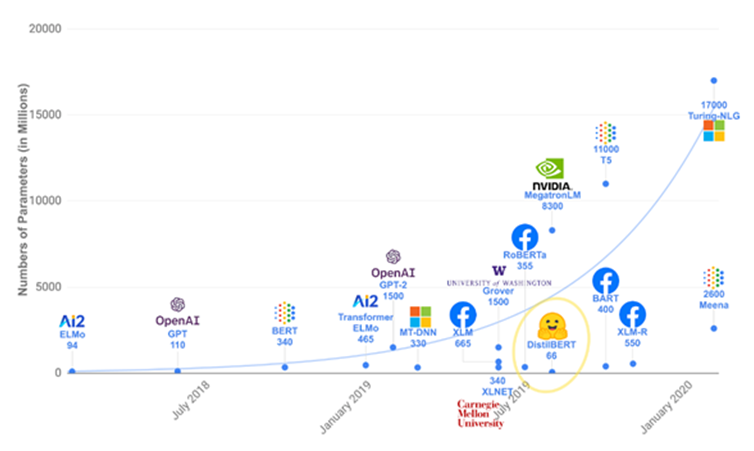
\includegraphics[width=0.7\linewidth]{fig1.png}
\caption{深度学习模型参数显著增长}
\label{fig-dl}
\end{figure}


研究人员表明,较大的模型会带来更高的准确性。
% 
从过去几年深度神经网络 (DNN) 驱动的机器学习技术的快速发展来看,研究者们发现加入更多 DNN 模型参数是最直接但不太复杂的方法之一提高 ML 算法的性能\ucite{kaplan2020scaling}。
% 
然而,DNN 模型容量通常受到计算资源和能源成本的限制\ucite{sharir2020cost}。
% 
根本原因是 DNN 的密集架构,其中计算成本通常与参数数量成线性比例。
% 
为了解决这种问题,混合专家 (MoE)~\ucite{lepikhin2020gshard} 在 DNN 中被广泛使用,它通过使用多个并行子模型(混合专家)引入了稀疏架构,其中每个输入经过门网络,动态选择并转发给少数专家处理。
% 
专家混合似乎有望将模型扩展到极端尺寸。
% 
如图\ref{fig-moe-training} 所示,与直接将小模型缩放为大密集模型不同,MoE\ucite{lepikhin2020gshard} 模型由许多小模型组成,即专家。
% 
训练样本被送入不同的专家,由轻量级可训练门网络动态选择。
% 
在 MoE 中,由于稀疏激活专家,节省了大量额外的计算量,与传统的密集型DNN相比,可以显着增加同一时间段内训练的样本数,提高模型精度。MoE技术是如今将DNN扩展到万亿参数的流行方法之一。

%
MoE混合专家系统是一种稀疏模型,因此其训练过程不同于传统的密集型DNN模型。主要有以下三点挑战:

\begin{itemize}
    \item 
    \textbf{动态激活特性:}
    MoE模型的稀疏激活特性使得它在GPU集群分布式训练时与现有的静态并行策略不匹配。
    因为MoE模型的每个样本只会被激活一个专家(也就是一个子模型),而其他的专家则不会被激活。
    这导致静态并行策略无法充分利用计算资源,因为只有部分计算节点被激活,而其他节点则处于空闲状态。
    % 因此,需要采用动态并行策略来适应MoE模型的稀疏激活特性,以最大限度地利用计算资源。

    \item 
    \textbf{额外通信开销:}
    MoE模型引入了GPU集群节点间额外的All-to-All通信,这种通信方式需要在所有计算节点之间进行数据传输和同步,由于All-to-All通信是一种同步通信方式,因此它会严重影响训练速度和效率。
    但是这种通信方式在MoE模型中是必需的,因为它需要将每个计算节点计算得到的结果进行汇总和组合,以得到最终的预测结果。
    % 为了减少All-to-All通信的开销,可以采用异步通信或一些优化策略,如节点划分和负载均衡,以提高通信效率和并行度。

    \item 
    \textbf{节点负载不均衡:}
    由于MoE模型中的Gating在训练过程中不断变化,因此数据可能被分配到不同的专家上,导致负载分配不平衡的问题。
    如果某些专家的负载过高,而其他专家的负载过低,就会导致训练时间的延长和模型性能的下降。
    因此,需要根据每个专家的激活情况和计算负载进行动态的数据分配和负载均衡,以确保每个专家的计算负载均衡,并最大限度地利用计算资源。
    % 可采用一些负载均衡算法,如动态调整负载均衡和任务分配策略,以实现动态负载均衡和高效的训练


\end{itemize}

现有的分布式训练框架\ucite{pytorch,deepspeed}对于其稀疏性的结构没有很好的支持,因此本次毕业设置拟设计一种更加高效的MoE训练框架,加速其分布式训练的过程,从而降低训练大规模的MoE模型架构的成本。

\begin{figure}[t!]
\vskip 2ex
\centering
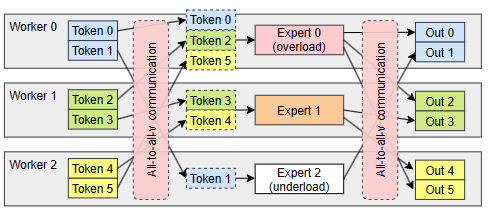
\includegraphics[width=0.69\linewidth]{fig6.png}
\caption{分布式MoE模型训练过程}
\label{fig-moe-training}
\end{figure}


\subsubsection{选题依据}
% 
随着人工智能技术的不断发展,MoE模型在各个领域都具有广泛的应用前景。它可以将多个不同的模型集成起来,以提高模型的性能和泛化能力。
% 
目前MoE模型在语音识别、自然语言处理、计算机视觉等领域都取得了很好的效果。
% 
因此,研究MoE模型的分布式训练和优化策略,可以进一步提高模型的训练效率和性能,适应更复杂和庞大的深度学习任务和数据集的需求。
% 
不仅能够为深度学习领域的研究提供新的思路和方法,还可以为各个领域的应用提供更加高效和精确的解决方案。



\section{研究内容}

\textbf{研究目标}。

\begin{figure}[t!]
    \vskip 2ex
    \centering
    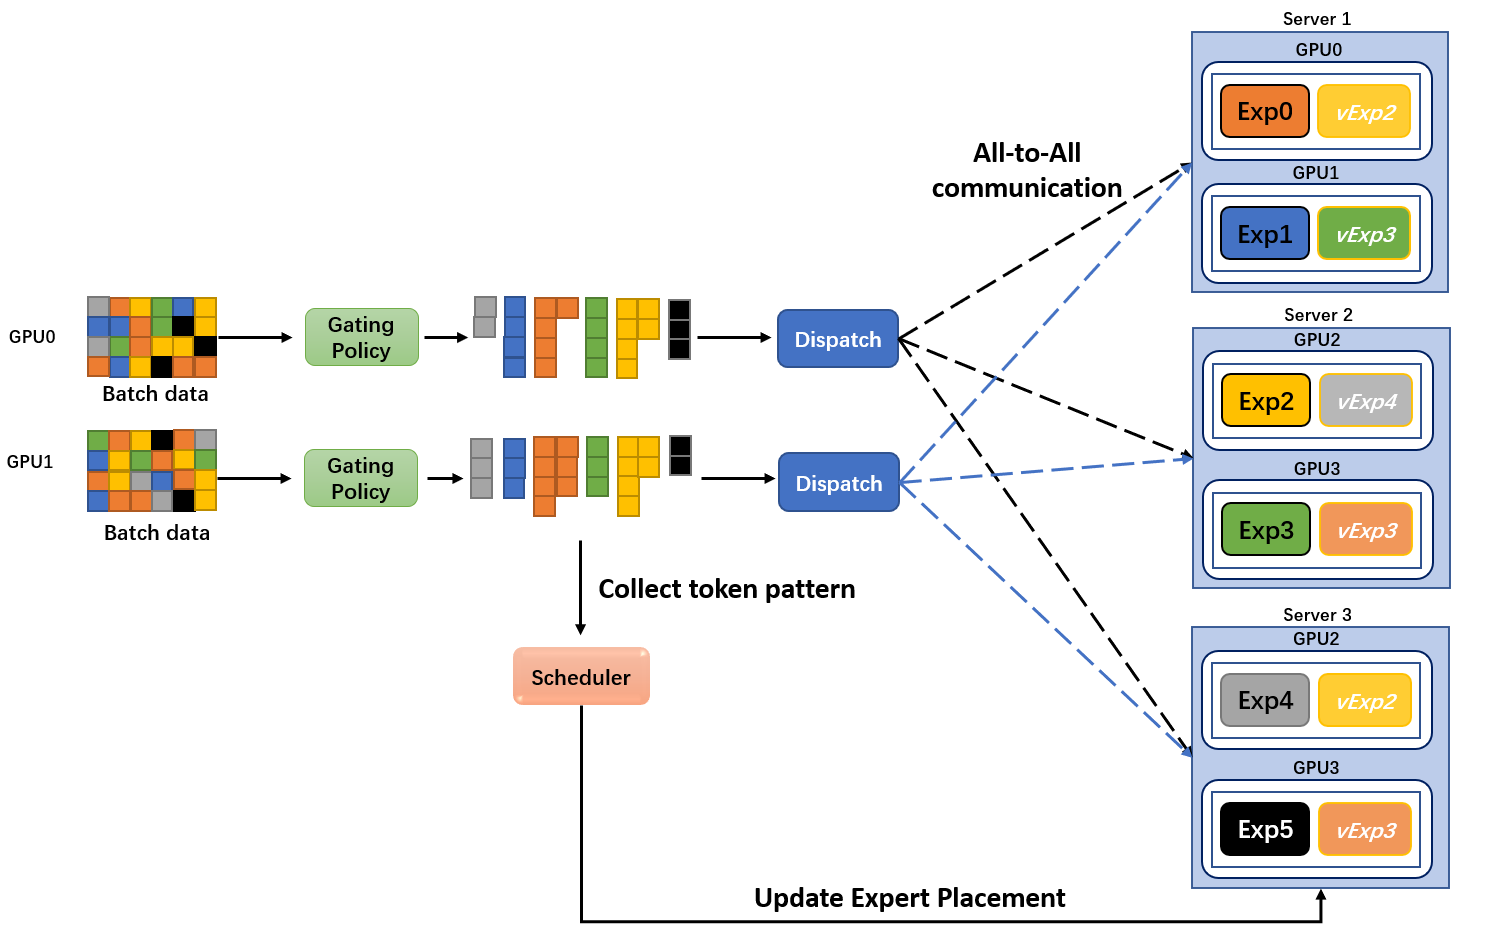
\includegraphics[width=0.99\linewidth]{figures/fig7.png}
    \caption{传统的Top1和Top2 Gating策略}
    \label{fig-overview}
    \end{figure}

本课题针对MoE模型带来以上挑战,拟分析现有的MoE模型分布式训练系统存在的缺陷,并设计一套全新的MoE模型训练系统。
% 
如图\ref{fig-overview}所示,我们提出了一种全新的MoE训练系统,通过在算法层面(gating policy)和系统层面(Expert placement scheduler)提出创新的训练解决方案,旨在克服MoE模型训练过程中的瓶颈,并更好地适应复杂而庞大的深度学习任务需求。

在算法层面,我们针对MoE模型的关键部分,即gating策略,进行了改进。我们通过动态调整数据分派策略,使其获得较快的收敛速度,同时也有合适的全局通信开销。

同时,在系统层面,我们提出了一种专家分配调度器(Expert placement scheduler),它能够根据网络拓扑以及任务负载,找到最合适的专家并行的策略。这样的设计考虑任务的特性、数据的分布以及专家的能力,我们能够动态地优化专家的分配策略,使得每个专家都能够发挥最大的潜力,并在整个系统中平衡负载和资源利用率。

这种全新的训练解决方案使得MoE模型能够更好地应对复杂和庞大的深度学习任务需求。通过优化算法和系统设计,我们能够充分发挥MoE模型的潜力,提高模型的准确性和泛化能力,为解决现实世界中的复杂问题提供了有力的工具。我们的研究对于推动MoE技术的发展和应用具有重要意义,并在深度学习模型训练的领域取得了显著的突破。

\subsection{基于动态路由的数据分派策略}

\begin{figure}[t!]
\vskip 2ex
\centering
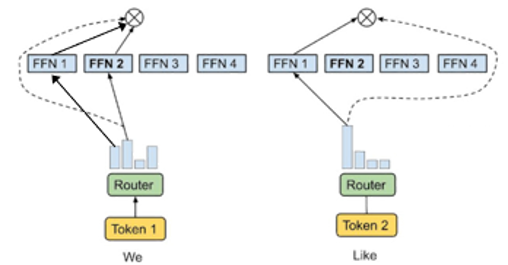
\includegraphics[width=0.5\linewidth]{figures/fig3.png}
\caption{传统的Top1和Top2 Gating策略}
\label{fig-top1_top2}
\end{figure}

如图\ref{fig-top1_top2}所示在传统的MoE模型中,采用固定的Top1和Top2 Gating策略,即将数据发送到分数最高(次高)的expert进行处理。
% 
然而,采用Top1 Gating时,由于只选择一个最高分数的expert,可能会错过其他有价值的信息,导致模型收敛速度较慢;
% 
而采用Top2 Gating时,虽然可以选择两个最高分数的expert,但每轮训练时间较长,因为需要进行两次All-to-All通信。
% 
因此我们能否将Top1和Top2 Gating策略结合起来,以一种动态的方式选择合适的数据分派策略,从而实现较快的收敛速度和较短的训练时间。
% 
一种简单的方法是,将每个数据按照Top1和Top2的分数进行排序,然后将它们分别分配给Top1和Top2的expert进行处理。
% 
这种方法可以利用Top1和Top2的优点,避免错过其他有价值的信息,同时减少通信开销,提高训练效率。

\subsection{基于网络拓扑的自动负载均衡策略}


\begin{figure}[t!]
\vskip 2ex
    \begin{minipage}[t]{0.48\linewidth}
        \centering
        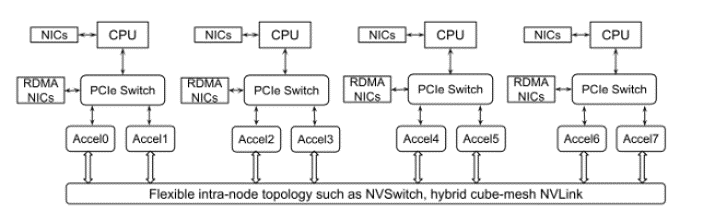
\includegraphics[width=1\linewidth]{figures/fig4.png}
        \caption{GPU集群内网络拓扑连接图}
        \label{fig-kek-tree}
    \end{minipage}
    %
    \begin{minipage}[t]{0.48\linewidth}
        \centering
        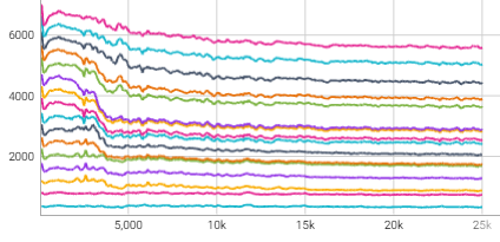
\includegraphics[width=0.8\linewidth]{figures/fig5.png}
        \caption{8层128专家的Transformer-XL\ucite{dai2019transformer}的MoE模型,第1层16个专家负载变化情况}
        \label{fig-transformer-xl}        
    \end{minipage}
\end{figure}

虽然基于 MoE 的算法开辟了一个巨大扩展模型参数量机会,但它也对训练系统带来了新的挑战,而这些挑战在之前的密集型DNN训练算法和系统中从未见过。根本原因是动态专家选择和灵活的 MoE 结构。具体来说,每个 MoE 层由一定数量的并行专家组成,这些专家分布在加速器(本工作中的 GPU)上,其中每个 GPU 根据智能门函数将每个输入数据分配给几个最适合的专家并取回相应的输出以将它们组合起来。这意味着每个专家的工作量基本上是不确定的,取决于输入数据和门函数。在图\ref{fig-transformer-xl}中,我们使用了一个8层的Transformer-xl MoE模型,分析了第1层16个专家负载变化情况。

我们发现,在MoE模型中,不同专家的负载在每次迭代中都会发生变化。
% 
这种现象是由于MoE的稀疏性动态数据分配所导致的,导致每个专家获取的数据不均匀,从而产生了负载不均衡的问题。
% 
这会导致一些节点或expert的负载过重,从而影响整个模型的训练速度和效果。因此,需要采取适当的负载均衡策略来缓解这个问题。
% 
此外在MoE模型中所有专家都需要从其他GPU上那里获得输入,这引入了GPU集群所有节点间额外的All-to-All通信,且All-to-All通信与后续计算是完全同步关系,并行较差。
% 
而GPU集群内部节点之间的网络带宽并不相同,节点通信效率存在差异。
% 
因而All-to-All通信也成为了大规模MoE训练中最耗时的操作之一。
% 
它通常实现为具有可变消息大小的同步 All-to-All 操作。考虑到动态特性的数据分派会导致计算和通信的严重不平衡,这样的方法会导致严重的开销。

因此,为了解决负载不均衡问题,需要采取一些适当的负载均衡策略,我们需要结合GPU集群内部节点之间的网络带宽不相同的情况,选择最佳的负载均衡策略,以提高整个模型的训练效率和性能。

% \medskip



\section{国内外研究现状}

\subsection{MoE训练系统}
随着MoE训练范式的普及,许多科研机构和企业都开源了MoE训练框架和系统。 
% 
DeepSpeed-MoE 利用多种分布式并行方法结合 MoE 并行性,包括数据并行、张量切片\ucite{shoeybi2019megatron}、Zero内存优化\ucite{rajbhandari2020zero}来训练更大的模型。至于 MoE 的推理,DeepSpeed\ucite{rajbhandari2022deepspeed}设计了一种名为 PR-MoE 的新型稀疏激活模型和模型压缩技术来减小 MoE 模型的大小,以及一种有效的通信方法来优化延迟。 
% 
FastMoE\ucite{he2021fastmoe} 是一个分布式 MoE 训练系统,它提供了一个分层接口和简单的机构,说明如何基于数据并行性和张量切片并行性使用 Megatron-LM\ucite{shoeybi2019megatron} 和 Transformer-XL\ucite{dai2019transformer}。
% 
与 DeepSpeed 的实施不同,FastMoE 使用复杂的优化方法来减少网络流量。
% 
Fairseq-MoE\ucite{ott2019fairseq}  是一个序列建模框架,用于训练用于摘要、翻译和语言建模的自定义模型。
% 
而 Tutel\ucite{hwang2022tutel} 在通信和计算方面进一步优化了 Fairseq 系统,其性能提升了约 40\%。
Tutel 中的优化已集成到 DeepSpeed 中,以促进 MoE 模型训练。

\subsection{MoE数据分派策略}
MoE的核心问题之一是如何设计gating策略,即如何根据输入分配不同的专家网络。不同的gating策略会影响模型的性能、稀疏性、均衡性和公平性。
\begin{itemize}
    \item Softmax gating\ucite{he2021fastmoe}:这是最简单的一种gating策略,它使用一个softmax层来为每个输入分配一个概率分布,表示每个专家网络的权重。这种方法可以看作是多个专家网络合作来产生输出,但是也会导致所有的专家网络都被激活,从而增加计算量和内存消耗。
    \item Top-k gating\ucite{hwang2022tutel}:这种gating策略只选择概率最高的k个专家网络来处理输入,其他的专家网络则被忽略。这种方法可以实现稀疏性,即只有少数的专家网络被激活,从而节省计算量和内存消耗。但是这种方法也会带来一些问题,比如如何确定k的值,以及如何保证每个专家网络都能被充分利用。
    \item Noisy softmax gating\ucite{xu2022survey}:这种gating策略在softmax gating的基础上增加了一个可学习的噪声权重,用来提高不同专家网络的gating均衡性。这种方法可以防止某些专家网络被过度使用或者被忽略,从而提高模型的公平性和泛化能力。
    \item Hierarchical softmax gating\ucite{xu2022survey}:这种gating策略将多个专家网络组织成一个层次结构,每一层都有一个softmax gating来决定下一层的激活。这种方法可以减少softmax gating的计算复杂度,从而提高模型的效率。
    \item Hash layer\ucite{roller2021hash}:这种gating策略使用哈希函数来为每个输入分配一个或多个专家网络,而不需要学习任何参数或者使用额外的损失函数。这种方法可以实现极高的稀疏性和效率,同时保持或者提升模型的性能。
    \item Topology-aware gating\ucite{chen2022ta}: TA-MoE中提出了一种拓扑感知的路由策略,它能够根据网络拓扑的变化动态地调整MoE的数据分派的调度策略。通过基于通信建模的方法,TA-MoE将调度问题抽象为一个优化目标,并得到了适用于不同拓扑结构的近似调度模式。他们设计了一种拓扑感知辅助损失函数,它可以自适应地根据底层拓扑调整数据分派策略,而不会牺牲模型的准确性。
\end{itemize}

\subsection{分布式深度学习训练系统概述}

分布式深度学习训练是一种将一个任务划分为较小的子任务并在多个处理器或设备上同时运行的技术\ucite{ben2019demystifying}。
% 
这种方法可以加快任务的执行速度,特别是当子任务可以在不同的处理器或设备上并行执行时。
% 
在分布式深度学习训练中,我们通过将训练数据和模型参数分布在多个处理器或设备上,然后在多个GPU上同时执行子任务来提高训练速度。
% 
这使我们能够突破单个GPU的内存限制,训练出比单个处理器或设备上所能训练的更大的深度学习模型。
% 
通过将训练过程在多个GPU上并行化,我们有效地增加了可用于训练模型的计算能力。每个GPU在训练数据的一个子集和模型参数的一部分上工作。然后通过汇总各个GPU的结果来建立整体模型。
% 
随着深度学习模型的规模和复杂性不断增加,分布式训练的好处变得更加明显。
% 
更大的神经网络需要更多的数据和计算来优化大量的权重和参数。
% 
通过利用多个GPU,我们可以扩大可用资源的规模,以满足这些大规模模型的需求。

目前,分布式深度学习训练中使用的并行性主要有三种类型:

\begin{itemize}
\item 
\textbf{数据并行性 (Data parallel)\ucite{ben2019demystifying}:}
在数据并行要求整个模型能够装入每个处理器或设备的内存中,这种方案将大规模的数据集分成多个小批次,分别在不同的处理器或设备上并行计算,以提高深度学习模型的训练速度和效率。
% 
在每个训练迭代或历时结束时,模型参数在所有处理器或设备上同步。
% 
更具体地说,每个处理器或设备在其训练数据部分的一批训练样本上工作。
% 
它在这个本地批次上执行前向和后向传播,以计算梯度并更新其模型副本中的权重和偏差。
% 
计算完成之后需要执行同步步骤,来自每个处理器或设备的模型参数被平均到一起(太频繁的同步会因为通信开销而降低训练速度,而太不频繁的同步则会导致独立的模型副本之间出现分歧)。
% 
通过数据并行和模型参数的定期同步,训练数据和计算可以有效地分布在多个处理器或设备上,以加快深度学习模型的训练。
% 
总的来说,数据并行难度相对较低,只需要并行化已有代码,但是其额外的通信开销随着GPU数量增加而增加,大规模训练性能较差。


\item
\textbf{模型并行性 (Model parallel)\ucite{shazeer2018mesh}:}
模型并行可用于训练太大而无法放入单个处理器或设备的内存中的模型,但是需要处理器或设备之间进行更多通信模型的参数分割到多个GPU卡或服务器上训练。
% 
这种方法将复杂的深度学习模型分割成独立的子模型,并分配到多张GPU卡或服务器上,从而减少单个设备的计算负担。
% 
在每张GPU计算完成对应部分之后,需要将中间的激活值通过网络传输(NCCL\ucite{nccl})的方式发送给其他GPU参与后续阶段参与计算。
% 
使用模型并行需要对模型进行重构以分割参数,因此相应的并行度比较高。
% 
这种方式可以利用更多的计算资源来加速非常大模型的训练,但是参数分割和同步亦需要投入额外工作并存在较高的通信开销。
% 
总的来说,模型并行适合那些模块化清晰且参数易于分割的深度学习模型,并且可以更好地随处理器数量线性缩放。


\item
\textbf{流水线并行 (Pipeline parallel)\ucite{huang2019gpipe}:}
流水线并行是一种通过将深度学习模型划分为多个独立阶段,并行执行不同阶段来加速训练模型的技术。具体操作包括:
% 
首先将模型分割成多个连续的阶段,如Embedding层、卷积层、池化层等
% 
并将一个Batch的数据划分为多个Macro-Batch分配给不同的阶段进行计算。
% 
当一个Macro-Batch通过一个阶段后,将结果传递给下个阶段,直至所有的Macro-batch通过流水线。
% 
不同阶段的计算可以同时执行,形成 computaional pipeline。
% 
整个Batch全部通过后,损失函数和梯度计算在最后一个阶段完成。
% 
流水线并行适用于很大的模型,超出单个GPU容量。它可以利用多个GPU来加速训练。
% 
流水线并行的优点是可以扩展到多个GPU来利用更多计算资源,利用计算资源更有效率。
% 
但是它主要挑战是需要更严格的同步不同阶段的计算,部分阶段可能存在空转,需要通过调整Macro-Batch大小来缓解。
% 
通常模型并行与流水线并行可能一起使用,以更好的平衡流水线并行中各个阶段的计算负载与数据通信开销。

\end{itemize}

并行训练模型时,我们需要通过合理的任务划分和调度来优化深度学习训练的效率和可扩展性,并根据深度学习模型本身的特点和可用的硬件资源选择最佳的并行方案。从而在保证模型精度的同时,实现训练速度提升,支持更大规模的训练,以及提高可靠性和容错性。
% 
这种方式可以更充分地利用计算资源,提高深度学习模型的训练效率和可扩展性,从而适应越来越复杂和庞大的深度学习任务和数据集的需求。

\section{本文组织结构}

本文的组织结构如下:

本文的第二章是MoE训练过程的概述。
% 
该章主要介绍了MoE混合专家模型在分布式深度学习训练中的主要过程,分析了其正向反向传播的计算过程,并解释了为什么MoE模型与现有传统集中式训练系统的不匹配。

本文的第三章是基于动态路由的数据分派策略的设计方式。
%
该章首先分析了现有的数据分派策略的主要方式,并总结了现有设计的不足之处。进而更进一步,给出了我们设计的基于动态路由的数据分派策略具体的方案架构,包括方案的详细流程和性能分析。


本文的第四章为基于网络拓扑的自动负载均衡策略方案设计。
%
该章首先分析了现有GPU数据中心网络拓扑。并结合每个专家在训练过程的负载变化现象,建立模型寻找最佳的负载均衡方案设计。


本文的第五章为系统实现以及实验结果展示。
%
该章给出了整体的设计方案以及实验结果展示。

本文的第六章为总结与展望。
%
该章总结了本文的主要贡献,以及对未来工作的展望。


\section{本章小结}

本章首先对论文选题的背景和研究意义进行讨论,提出了稀疏混合专家MoE模型对于现有深度学习训练系统的挑战,然后分别介绍了本文的研究点。
%
随后对国内外研究现状进行了简要的介绍。

\endinput
\chapter{MoE模型训练过程概述}

MoE模型在原本Transformer block的FFN中通过添加门控函数以及一系列相互并列的专家组成。
% 
在训练过程中门控函数主要将输入数据分配给不同的专家模型参与前向/反向计算,这一过程主要通过All-to-All通信实现。
% 
待每个专家计算完成相对应的数据之后,我们需要通过一次额外的All-to-All通信,将计算完成的激活值返回原本对应的GPU上,并参与后续的计算过程。

\section{MoE模型的分布式训练}

\begin{figure}[h!]
    \vskip 2ex
    \centering
    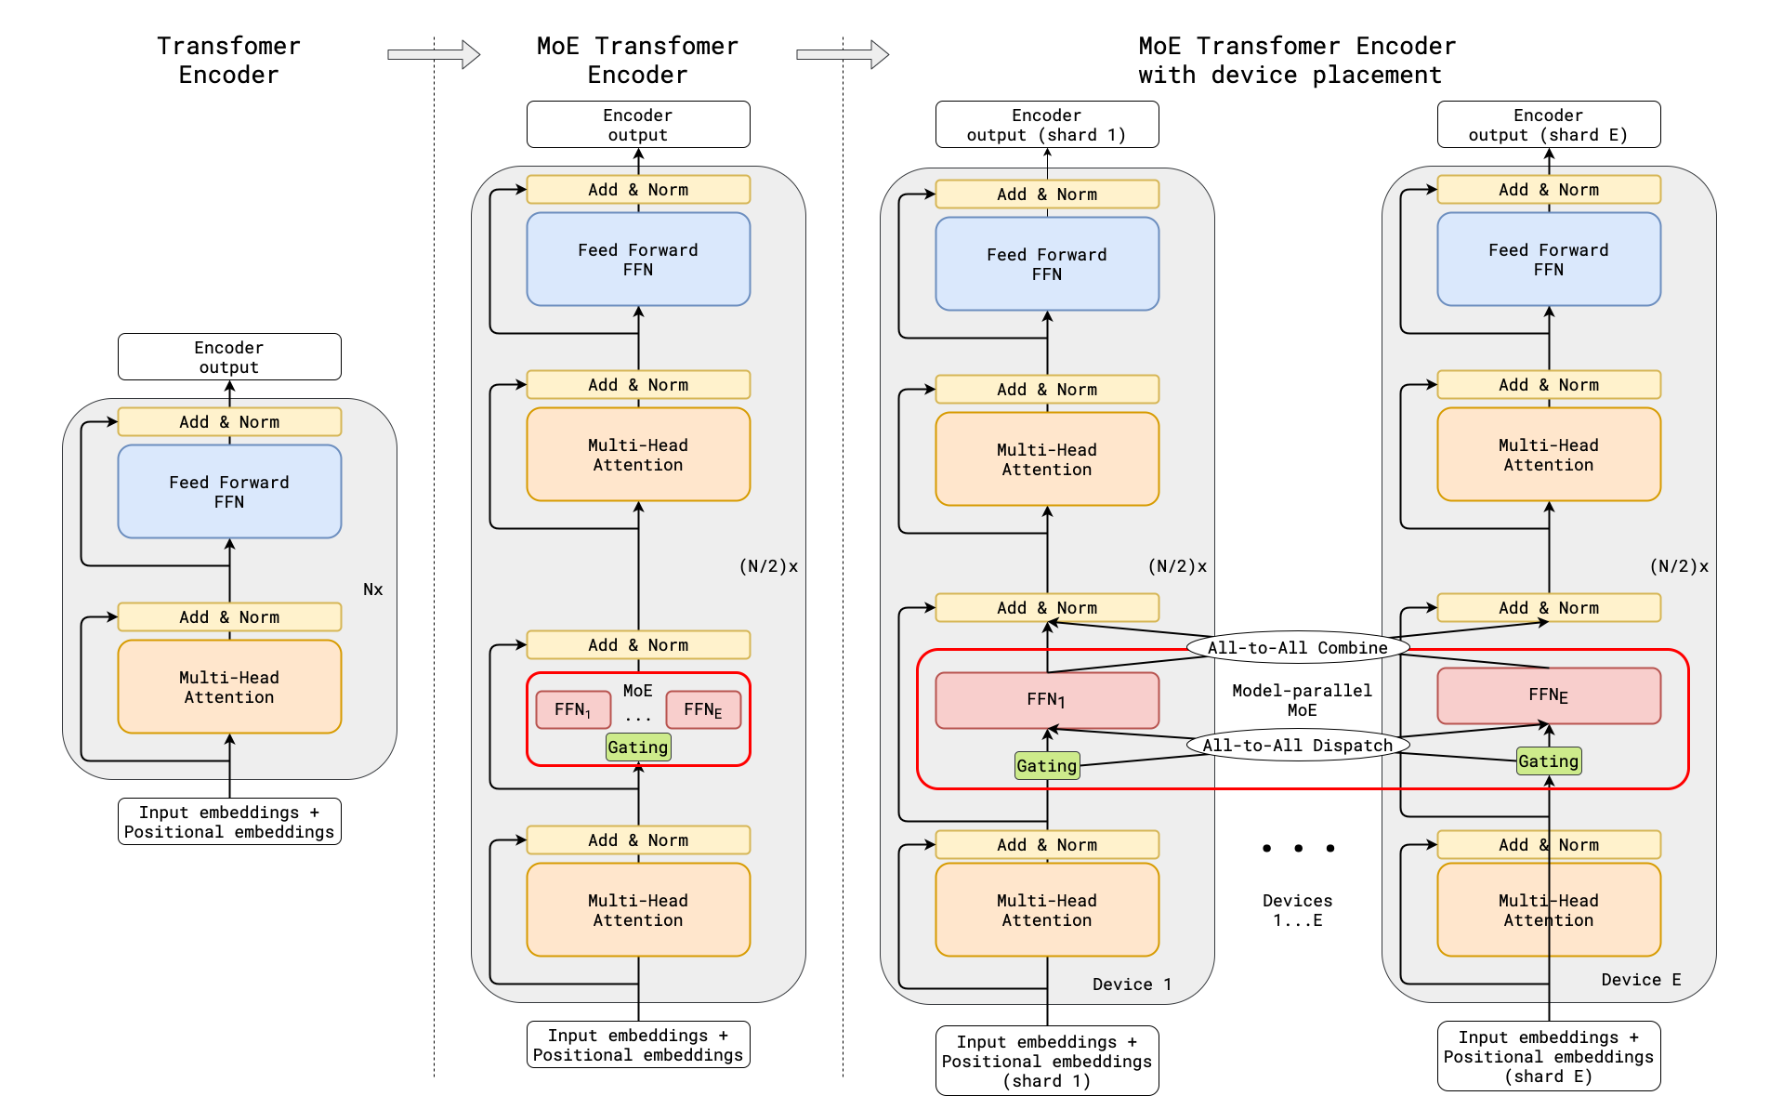
\includegraphics[width=0.99\linewidth]{figures/fig2.png}
    \caption{MoE模型训练过程}
    \label{fig-moe-arch}
    \end{figure}

图\ref{fig-moe-arch}展示了传统的集中式的Transformer模型训练过程转变到分布式的Transformer-MoE训练过程的示意图。
% 
绿色的部分是增加的门控函数,用于决定将数据分派至哪一个expert参与计算,红色部分的$\mathbf{FFN_1-FFN_E}$表示该层中具有E个互相独立的专家个数。
% 
由于GPU的显存有限,不能将所有的专家的参数都在一张GPU中保存下。
% 
因此GShard\ucite{lepikhin2020gshard}的研究者们提出了专家并行的概念,将每个专家的参数单独放置在GPU上,其他部分采用数据并行的架构,从而实现了一种混合的分布式训练过程。
% 
在训练过程结束之后,通常需要额外的All-reduce用于同步数据并行模块的梯度,最后根据每个可训练参数的梯度,调用优化器更新参数。

整体的训练流程总结如下:

\begin{itemize}

    \item \textbf{1.数据划分}
    
每个GPU将训练数据随机筛选,确保每一轮训练中每个GPU上包含的数据子集是互不重复的。
% 
每个子集分配到不同的GPU或计算节点上进行训练。
    
    \item \textbf{2.数据并行\&专家并行}
    
在MoE模型训练中,数据并行和专家并行通常结合使用,以实现更高效的分布式训练。
% 
具体而言,可以将训练数据划分为多个子集,并将每个子集分配到不同的GPU或计算节点上。
% 
在每个GPU或计算节点上,可以使用专家并行的方式对每个专家模型进行训练,同时使用数据并行的方式对整个MoE模型进行训练。
% 
这样可以将计算负载和数据负载都分散到多个GPU或计算节点上,从而加速整个MoE模型的训练过程。

    \item \textbf{3.前向传播}
    
    每一层的前向传播主要在以下两个步骤区别与传统的密集型Transformer计算。(数据分派和专家计算)。

在数据分派阶段,MoE模型使用Gating门函数对每个输入数据进行加权打分,以决定每个专家模型的贡献。这个Gating函数由一层MLP和softmax组成。具体而言,MoE模型将输入$x$输入到门控模型中,得到一个$E$维的得分,$f=[f_1,f_2,\cdots,f_E]$, $f_i$表示第$i$个专家模型的权重得分。门控向量的每个元素都是非负的,并且它们的和等于1,即$\sum_{i=1}^K g_i = 1$。最后通过全局所有GPU的All-to-All通信,将对应数据发送给相应的GPU,参与后续的计算。

专家计算阶段,每个GPU上接收到其他GPU传输来的数据后(假设有d维),将其输入相应的专家模型参与前向计算。
% 
得到d维的输出向量$r$。之后通过反向的All-to-All通信,将激活值返回对应的GPU上,得到每个GPU上原本数据的输出向量$z=[z_1,z_2,\cdots,z_E]$。
% 
然后,MoE模型将每个输出向量$z_i$与对应的门控向量$g_i$进行按元素乘法,得到一个加权输出向量$w$,其中$w_{i}=g_{i}z_{i}$。最后,MoE模型将所有加权输出向量$w_i$进行累加,得到最终的输出向量$y$,其中$y=\sum_{i=1}^E w_{i}$。

    \item \textbf{4.反向传播}
    
    是用于计算MoE模型的梯度,其过程类似于传统的神经网络模型。
    % 
    在完成前向传播计算之后,使用PyTorch的自动求导机制(autograd)建立计算图,并自动计算每个参数的梯度。
    % 
    具体而言,可以使用loss函数对模型的输出进行评估,并计算输出和目标值之间的误差。
    % 
    然后,使用误差及其对模型参数的导数,计算每个参数的梯度。
    % 
    反向传播过程可以使用链式法则(chain rule)实现,即将误差从输出层向输入层传播,并依次计算每个参数的梯度。

    \item \textbf{5.梯度计算}
    
    是将每个模型的梯度进行同步,以便在参数更新时使用。
    % 
    由于MoE模型的分布式训练过程涉及多个GPU或计算节点的并行计算,因此需要使用all-reduce等方法将所有模型的梯度进行同步。

    \item \textbf{6.参数更新}
    
    使用优化器对模型参数进行更新,以最小化损失函数。在MoE模型训练中,可以使用常见的优化器,如Adam、SGD等,对每个模型的参数进行更新。
    % 
    通常,参数更新的速率会受到学习率(learning rate)等超参数的控制,以平衡模型的收敛速度和稳定性。

    \item \textbf{7.重复迭代}
    
    将以上步骤重复多次,直到模型收敛为止。在每次迭代中,可以使用不同的训练数据子集,防止模型陷入局部最优解。

\end{itemize}

\section{MoE训练瓶颈分析}

在GPU集群中分布式训练MoE模型时,我们首先测量分析了一些已有训练系统存在的缺陷和问题,这些挑战会极大地影响训练效率。

\begin{table}[]
    \centering
    \label{table-moti}
    \caption{使用Transformer-xl~\ucite{dai2019transformer}语言模型再不同模型设计下的All-to-All通信时间与每个训练阶段完成时间。每个FFN层都使用MoE替代,且专家的数量等于GPU的数量。}
\begin{tabular}{ccccc}
\hline
\cellcolor[HTML]{FFFFFF}\#Experts & Model      & All-to-All & Step Time & Ratio                           \\ \hline
                                  & 8L + 94M   & 259        & 722       & \cellcolor[HTML]{FFFFFF}35.80\% \\
                                  & 12L + 117M & 589        & 1684      & \cellcolor[HTML]{FFFFFF}34.90\% \\
\multirow{-3}{*}{4}               & 24L + 233M & 1479       & 3894      & \cellcolor[HTML]{FFFFFF}37.80\% \\ \hline
\end{tabular}
    \end{table}



\noindent \textbf{All-to-All通信效率低}
MoE模型的训练瓶颈之一是All-to-All通信,这是由于模型中多个专家模型之间需要进行信息交换所导致的。之前的工作已经确定了All-to-All通信是MoE模型训练的一个瓶颈~\ucite{he2021fastmoe,hwang2022tutel,li2023accelerating}。表2-1显示了在我们的GPU集群中各种语言模型的训练步骤时间以及All-to-All操作的完成时间。平均而言,All-to-All操作占用了37.4\%的步进时间,这是很大一部分。在下文中,我们通过剖析MoE中All-to-All通信成本的主要原因来引入我们的工作。我们的分析基于专家数量与(GPU)设备数量相同的常见场景。

首先,All-to-All操作是同步操作,会阻塞计算过程。图\ref{fig-moe-arch}显示了集群中MoE模型训练前向传递的流程图。我们观察到专家的FFN计算和组合操作仅在All-to-All操作完成时发生。在此期间,GPU大部分处于空闲状态。我们使用PyTorch Profiler对表2-1中每个实验中20个步骤的GPU活动进行了分析,并发现这种空闲状态很明显。在MoE模型的前向传递中,会使用两个All-to-All操作,一个用于将标记从之前的Add \& Norm层输出结果路由到选择的专家,另一个用于在专家计算后将它们发送回其原始GPU。因此,一个MoE层的完整训练步骤将涉及四个All-to-All操作,其中两个来自反向传递。这加剧了MoE模型训练的低效率问题。

其次MoE训练过程瓶颈的第二个原因是其庞大的数据传输规模。
由于专家的FFN架构确保其输入数据大小与输出数据大小相同,因此前向传递的两个All-to-All操作中的数据传输具有相同的大小。
数据传输的大小由每个GPU的\textit{batch\_size}、专家(或GPU)的数量N、序列长度\textit{seq\_len}, 如top-k中的k(所选专家的数量)以及编码器,解码器输入\textit{d\_model}中的特征大小决定。

\section{本章小结}

本章我们主要分析了现有的MoE模型训练过程,MoE模型的训练过程通常比传统的神经网络模型更为复杂和耗时,需要充分利用分布式计算和并行计算等技术,以提高训练速度和效率。
% 
同时,MoE模型的设计和调整也需要考虑多个因素,如门控模型的设计、专家模型的选择和训练方式等,以提高模型的性能和泛化能力。

\endinput
\chapter{基于智能合约的加密数据去重方案设计}

\section{区块链的公开特性}

\section{加密数据去重方案概述}

\subsection{系统构成}

\subsection{威胁模型及假设}

\subsection{方案设计要求}

\section{加密数据去重方案架构设计}

\subsection{数据结构及函数}

\subsection{加密去重详细流程}

\subsection{安全性分析}

\section{本章小结}

\endinput
\chapter{面向加密数据去重的动态用户更变方案设计}

\section{动态用户更变方案概述}

\subsection{系统构成}

\subsection{威胁模型及假设}

\subsection{方案设计要求}

\section{动态用户更变方案架构设计}

\subsection{符号定义及概念}

\subsection{用户更变详细流程}

\subsection{安全性分析}

\section{本章小结}

\endinput
\chapter{基于通信延迟的地理位置验证方案设计}

\section{地理位置验证方案概述}

\subsection{节点距离估计}

\subsection{基本测量流程}

\section{地理位置验证方案架构设计}

\subsection{验证方案框架详细流程}
% \subsection{多节点测距}

% \subsection{测量结果广播}

% \subsection{迭代验证}

\subsection{结果置信度计算}

\section{本章小节}

\endinput
\chapter{系统测试与分析}

\section{系统测试环境}

我们的系统基于 Microsoft 开源的 Deepspeed 框架 \ucite{deepspeed} 进行开发,主要使用 Python 语言。我们使用了一个 8 层的 Transformer-xl 模型 \ucite{dai2019transformer},并在其基础上拓展成为 MoE 架构。
在数据集的选择上,我们主要使用了 enwik8 数据集 \ucite{enwik8} 进行测试。

我们使用了私有集群进行测试,其中包括两种不同的 GPU 集群配置,用于验证基于网络拓扑的自动负载均衡策略设计。我们主要使用了 2 节点 8 卡的 Nvidia Titan XP GPU 集群以及 4 节点 8 卡的 Nvidia Titan XP GPU 集群。集群节点之间的网络通信通过Ethernet,其带宽约为10Gb/s。

\section{系统性能指标}

我们主要关注两个性能指标进行测试。第一个指标是模型的收敛速度,即 loss 收敛速度。第二个指标是每个 step 的完成时间,即模型训练过程中每个batch所需要的forward + backward + gradient synchronization所需要的总时间。我们将对这两个指标进行详细的测试评估,并根据测试结果进行优化和调整。

\section{实验结果}

\subsection{动态路由的数据分派策略实验结果}

我们进行了动态路由的数据分派策略实验,并将我们的设计与传统的Top-1和Top-2 Gating策略进行了对比。实验的对象是Transformer-XL模型,我们关注了每轮训练中损失的变化情况,并将其可视化为图表。

\begin{figure}[h!]
    \vskip 2ex
    \centering
    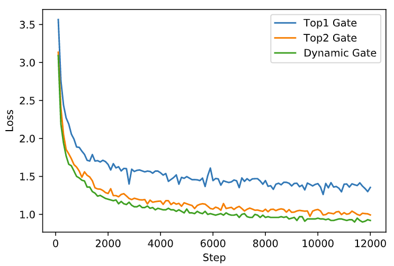
\includegraphics[width=0.7\linewidth]{figures/fig9.png}
    \caption{训练Loss变化图}
    \label{fig-loss}
    \end{figure}

    对比传统的Top-1和Top-2 Gating策略,我们的设计采用了动态路由的数据分派策略。通过实验结果的对比分析,我们发现我们的设计在损失的降低速度和最终的收敛效果上表现出了显著的优势。图\ref{fig-loss}清晰地展示了每轮训练中损失的变化趋势,我们的设计在较早的轮次就取得了更快的收敛速度,并且在后续的训练过程中持续保持较低的损失值。

这些实验结果表明,我们的动态路由数据分派策略在Transformer-XL模型上的有效性和优越性。相比传统的Top-1和Top-2 Gating策略,我们的设计能够更好地调度和分配数据,使得模型能够更快地收敛并获得更好的训练效果。这为提升模型性能和训练效率提供了有力的实证支持。

综上所述,我们的动态路由数据分派策略在Transformer-XL模型上的实验结果显示出了明显的优势,为改进模型训练和优化数据分派提供了一种有效的方法。这些发现对于深度学习研究和实践具有重要意义,并为未来的工作和改进方向提供了有益的启示。

\subsection{基于网络拓扑的自动负载均衡实验结果}

\subsubsection{端到端训练性能分析}
我们对基于网络拓扑的自动负载均衡设计在GPU集群上进行了测试,我们使用了2个节点,每个节点配备了8个Nvidia TitanX GPU。网络带宽为10Gbps,训练框架采用了Deepspeed,MoE模型为Transformer-xl MoE,数据集为enwik8,模型参数量为45M。

根据我们的实验数据\ref{fig-breakdown},我们的设计在前向传播阶段获得了约4.09倍的加速比。这表明我们基于网络拓扑的自动负载均衡设计在模型的前向计算过程中取得了显著的性能提升。通过有效地分配计算任务和利用GPU集群的并行能力,我们能够加快前向传播的速度,从而加速整体训练过程。

\begin{figure}[h!]
    \vskip 2ex
    \centering
    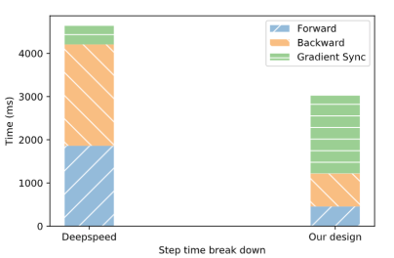
\includegraphics[width=0.7\linewidth]{figures/fig10.png}
    \caption{参数量为45M时,每个step时间步分解}
    \label{fig-breakdown}
    \end{figure}

在后向传播阶段,我们的设计获得了约3.08倍的加速比。这进一步证明了我们的自动负载均衡设计在处理梯度计算和参数更新时的优越性。通过合理地分配计算任务和优化通信流程,我们能够有效地利用GPU集群的计算资源,提高后向传播的效率。

然而,在梯度同步阶段,由于更负载的并行策略和更复杂的通信流程,我们的设计可能会遇到一定程度的性能下降。这是因为梯度同步过程中的通信开销增加,可能导致整体训练速度的一定减缓。

综合而言,基于我们的实验结果,我们的基于网络拓扑的自动负载均衡设计在前向传播和后向传播阶段分别获得了约4.09倍和3.08倍的加速比。虽然在梯度同步阶段可能存在一定的性能下降,但最终整体端到端的训练速度仍然提升了约1.24倍。这证明了我们设计的有效性和优越性,能够加速训练过程并提高模型训练的效率。在未来的工作中,我们将继续优化和改进设计,以进一步提高整体训练速度并减少梯度同步阶段的性能下降。

\begin{table}[]
    \centering
    \label{table-45M}
    \caption{在参数量为45M的Trasnformer-xl MoE模型训练中,我们的设计与baseline(Deepspeed)的Step Time的拆分}
    \begin{tabular}{|
    >{\columncolor[HTML]{FFFFFF}}l |
    >{\columncolor[HTML]{FFFFFF}}l |
    >{\columncolor[HTML]{FFFFFF}}l |
    >{\columncolor[HTML]{FFFFFF}}l |}
    \hline
    {\color[HTML]{333333} Stages}             & {\color[HTML]{333333} Baseline} & {\color[HTML]{333333} Our design} & {\color[HTML]{333333} \textbf{Acc}}   \\ \hline
    {\color[HTML]{333333} Fwd\_MoE (ms)} & {\color[HTML]{333333} 1860} & {\color[HTML]{333333} 455}  & {\color[HTML]{333333} \textbf{4.09x}} \\ \hline
    {\color[HTML]{333333} Bwd\_Moe (ms)} & {\color[HTML]{333333} 2347} & {\color[HTML]{333333} 761}  & {\color[HTML]{333333} \textbf{3.08x}} \\ \hline
    {\color[HTML]{333333} Gradient Sync (ms)} & {\color[HTML]{333333} 430}      & {\color[HTML]{333333} 1805}       & {\color[HTML]{333333} \textbf{0.24x}} \\ \hline
    {\color[HTML]{333333} Overall (ms)}  & {\color[HTML]{333333} 5200} & {\color[HTML]{333333} 3576} & {\color[HTML]{333333} \textbf{1.45x}} \\ \hline
    \end{tabular}
    \end{table}

\subsubsection{自动负载均衡策略深入分析}

\begin{sidewaystable}
    \centering
    \begin{adjustbox}{max width=0.8\textwidth}
        \begin{tabular}{@{}|
            >{\columncolor[HTML]{FFFFFF}}l 
            >{\columncolor[HTML]{FFFFFF}}l 
            >{\columncolor[HTML]{FFFFFF}}l 
            >{\columncolor[HTML]{FFFFFF}}l |
            >{\columncolor[HTML]{FFFFFF}}l 
            >{\columncolor[HTML]{FFFFFF}}l 
            >{\columncolor[HTML]{FFFFFF}}l 
            >{\columncolor[HTML]{FFFFFF}}l 
            >{\columncolor[HTML]{FFFFFF}}l 
            >{\columncolor[HTML]{FFFFFF}}l 
            >{\columncolor[HTML]{FFFFFF}}l 
            >{\columncolor[HTML]{FFFFFF}}l 
            >{\columncolor[HTML]{FFFFFF}}l |@{}}
            \toprule
            \multicolumn{2}{|l|}{\cellcolor[HTML]{FFFFFF}{\color[HTML]{333333} 8 GPUs 2 Nodes}} &
              \multicolumn{2}{l|}{\cellcolor[HTML]{FFFFFF}model: transformer-xl} &
              \multicolumn{2}{l|}{\cellcolor[HTML]{FFFFFF}layer:8} &
              \multicolumn{2}{l|}{\cellcolor[HTML]{FFFFFF}batch\_size: 24} &
              \multicolumn{5}{l|}{\cellcolor[HTML]{FFFFFF}} \\ \midrule
            \multicolumn{1}{|l|}{\cellcolor[HTML]{FFFFFF}} &
              \multicolumn{3}{l|}{\cellcolor[HTML]{FFFFFF}Fwd\_MoE(ms)} &
              \multicolumn{3}{l|}{\cellcolor[HTML]{FFFFFF}Bwd\_inner(ms)} &
              \multicolumn{3}{l|}{\cellcolor[HTML]{FFFFFF}Bwd\_Allreduce (ms)} &
              \multicolumn{3}{l|}{\cellcolor[HTML]{FFFFFF}Overall (ms)} \\ \cmidrule(l){2-13} 
            \multicolumn{1}{|l|}{\multirow{-2}{*}{\cellcolor[HTML]{FFFFFF}\#Params}} &
              \multicolumn{1}{l|}{\cellcolor[HTML]{FFFFFF}Baseline} &
              \multicolumn{1}{l|}{\cellcolor[HTML]{FFFFFF}Our   design} &
              Acc &
              \multicolumn{1}{l|}{\cellcolor[HTML]{FFFFFF}Baseline} &
              \multicolumn{1}{l|}{\cellcolor[HTML]{FFFFFF}Our   design} &
              \multicolumn{1}{l|}{\cellcolor[HTML]{FFFFFF}Acc} &
              \multicolumn{1}{l|}{\cellcolor[HTML]{FFFFFF}Baseline} &
              \multicolumn{1}{l|}{\cellcolor[HTML]{FFFFFF}Our   design} &
              \multicolumn{1}{l|}{\cellcolor[HTML]{FFFFFF}Acc} &
              \multicolumn{1}{l|}{\cellcolor[HTML]{FFFFFF}Baseline} &
              \multicolumn{1}{l|}{\cellcolor[HTML]{FFFFFF}Our   design} &
              Acc \\ \midrule
            \multicolumn{1}{|l|}{\cellcolor[HTML]{FFFFFF}45M} &
              \multicolumn{1}{l|}{\cellcolor[HTML]{FFFFFF}1860} &
              \multicolumn{1}{l|}{\cellcolor[HTML]{FFFFFF}455} &
              \textbf{4.09x} &
              \multicolumn{1}{l|}{\cellcolor[HTML]{FFFFFF}2347} &
              \multicolumn{1}{l|}{\cellcolor[HTML]{FFFFFF}761} &
              \multicolumn{1}{l|}{\cellcolor[HTML]{FFFFFF}\textbf{3.08x}} &
              \multicolumn{1}{l|}{\cellcolor[HTML]{FFFFFF}430} &
              \multicolumn{1}{l|}{\cellcolor[HTML]{FFFFFF}1805} &
              \multicolumn{1}{l|}{\cellcolor[HTML]{FFFFFF}\textbf{0.24x}} &
              \multicolumn{1}{l|}{\cellcolor[HTML]{FFFFFF}5200} &
              \multicolumn{1}{l|}{\cellcolor[HTML]{FFFFFF}3576} &
              \textbf{1.45x} \\ \midrule
            \multicolumn{1}{|l|}{\cellcolor[HTML]{FFFFFF}94M} &
              \multicolumn{1}{l|}{\cellcolor[HTML]{FFFFFF}1929} &
              \multicolumn{1}{l|}{\cellcolor[HTML]{FFFFFF}463} &
              \textbf{4.17x} &
              \multicolumn{1}{l|}{\cellcolor[HTML]{FFFFFF}2386} &
              \multicolumn{1}{l|}{\cellcolor[HTML]{FFFFFF}815} &
              \multicolumn{1}{l|}{\cellcolor[HTML]{FFFFFF}\textbf{2.93x}} &
              \multicolumn{1}{l|}{\cellcolor[HTML]{FFFFFF}430} &
              \multicolumn{1}{l|}{\cellcolor[HTML]{FFFFFF}5350} &
              \multicolumn{1}{l|}{\cellcolor[HTML]{FFFFFF}\textbf{0.08x}} &
              \multicolumn{1}{l|}{\cellcolor[HTML]{FFFFFF}5161} &
              \multicolumn{1}{l|}{\cellcolor[HTML]{FFFFFF}7005} &
              \textbf{0.74x} \\ \bottomrule
        \end{tabular}
    \end{adjustbox}
    \label{table-dive-deep-param}
    \caption{更改模型参数,分析系统训练性能}
    
% \end{sidewaystable}

\bigskip
% \begin{sidewaystable}
    \centering
    \begin{adjustbox}{max width=0.8\textwidth}
        \begin{tabular}{@{}|
            >{\columncolor[HTML]{FFFFFF}}c 
            >{\columncolor[HTML]{FFFFFF}}c 
            >{\columncolor[HTML]{FFFFFF}}c 
            >{\columncolor[HTML]{FFFFFF}}c |
            >{\columncolor[HTML]{FFFFFF}}c 
            >{\columncolor[HTML]{FFFFFF}}c 
            >{\columncolor[HTML]{FFFFFF}}c 
            >{\columncolor[HTML]{FFFFFF}}c 
            >{\columncolor[HTML]{FFFFFF}}c 
            >{\columncolor[HTML]{FFFFFF}}c 
            >{\columncolor[HTML]{FFFFFF}}c 
            >{\columncolor[HTML]{FFFFFF}}c 
            >{\columncolor[HTML]{FFFFFF}}c |@{}}
            \toprule
            \multicolumn{2}{|c|}{\cellcolor[HTML]{FFFFFF}{\color[HTML]{333333} \textbf{8 GPUs 2 Nodes}}} &
              \multicolumn{2}{c|}{\cellcolor[HTML]{FFFFFF}\textbf{model: transformer-xl}} &
              \multicolumn{2}{c|}{\cellcolor[HTML]{FFFFFF}\textbf{layer:8}} &
              \multicolumn{2}{c|}{\cellcolor[HTML]{FFFFFF}\textbf{batch\_size: 40}} &
              \multicolumn{5}{l|}{\cellcolor[HTML]{FFFFFF}} \\ \midrule
            \multicolumn{1}{|c|}{\cellcolor[HTML]{FFFFFF}} &
              \multicolumn{3}{c|}{\cellcolor[HTML]{FFFFFF}Fwd\_MoE (ms)} &
              \multicolumn{3}{c|}{\cellcolor[HTML]{FFFFFF}Bwd\_inner (ms)} &
              \multicolumn{3}{c|}{\cellcolor[HTML]{FFFFFF}Bwd\_Allreduce (ms)} &
              \multicolumn{3}{c|}{\cellcolor[HTML]{FFFFFF}Overall (ms)} \\ \cmidrule(l){2-13} 
            \multicolumn{1}{|c|}{\multirow{-2}{*}{\cellcolor[HTML]{FFFFFF}\#Params}} &
              \multicolumn{1}{c|}{\cellcolor[HTML]{FFFFFF}Baseline} &
              \multicolumn{1}{c|}{\cellcolor[HTML]{FFFFFF}Our design} &
              Acc &
              \multicolumn{1}{c|}{\cellcolor[HTML]{FFFFFF}Baseline} &
              \multicolumn{1}{c|}{\cellcolor[HTML]{FFFFFF}Our design} &
              \multicolumn{1}{c|}{\cellcolor[HTML]{FFFFFF}Acc} &
              \multicolumn{1}{c|}{\cellcolor[HTML]{FFFFFF}Baseline} &
              \multicolumn{1}{c|}{\cellcolor[HTML]{FFFFFF}Our design} &
              \multicolumn{1}{c|}{\cellcolor[HTML]{FFFFFF}Acc} &
              \multicolumn{1}{c|}{\cellcolor[HTML]{FFFFFF}Baseline} &
              \multicolumn{1}{c|}{\cellcolor[HTML]{FFFFFF}Our design} &
              Acc \\ \midrule
            \multicolumn{1}{|c|}{\cellcolor[HTML]{FFFFFF}45M} &
              \multicolumn{1}{c|}{\cellcolor[HTML]{FFFFFF}3233} &
              \multicolumn{1}{c|}{\cellcolor[HTML]{FFFFFF}527} &
              \textbf{6.13x} &
              \multicolumn{1}{c|}{\cellcolor[HTML]{FFFFFF}4171} &
              \multicolumn{1}{c|}{\cellcolor[HTML]{FFFFFF}1146} &
              \multicolumn{1}{c|}{\cellcolor[HTML]{FFFFFF}\textbf{3.64x}} &
              \multicolumn{1}{c|}{\cellcolor[HTML]{FFFFFF}430} &
              \multicolumn{1}{c|}{\cellcolor[HTML]{FFFFFF}1813} &
              \multicolumn{1}{c|}{\cellcolor[HTML]{FFFFFF}\textbf{0.24x}} &
              \multicolumn{1}{c|}{\cellcolor[HTML]{FFFFFF}8365} &
              \multicolumn{1}{c|}{\cellcolor[HTML]{FFFFFF}4674} &
              \textbf{1.79x} \\ \midrule
            \multicolumn{1}{|c|}{\cellcolor[HTML]{FFFFFF}94M} &
              \multicolumn{1}{c|}{\cellcolor[HTML]{FFFFFF}3276} &
              \multicolumn{1}{c|}{\cellcolor[HTML]{FFFFFF}612} &
              \textbf{5.35x} &
              \multicolumn{1}{c|}{\cellcolor[HTML]{FFFFFF}3945} &
              \multicolumn{1}{c|}{\cellcolor[HTML]{FFFFFF}1250} &
              \multicolumn{1}{c|}{\cellcolor[HTML]{FFFFFF}\textbf{3.16x}} &
              \multicolumn{1}{c|}{\cellcolor[HTML]{FFFFFF}430} &
              \multicolumn{1}{c|}{\cellcolor[HTML]{FFFFFF}5350} &
              \multicolumn{1}{c|}{\cellcolor[HTML]{FFFFFF}\textbf{0.08x}} &
              \multicolumn{1}{c|}{\cellcolor[HTML]{FFFFFF}8168} &
              \multicolumn{1}{c|}{\cellcolor[HTML]{FFFFFF}7590} &
              \textbf{1.08x} \\ \midrule
            \multicolumn{1}{|c|}{\cellcolor[HTML]{FFFFFF}145M} &
              \multicolumn{1}{c|}{\cellcolor[HTML]{FFFFFF}3212} &
              \multicolumn{1}{c|}{\cellcolor[HTML]{FFFFFF}2145} &
              \textbf{1.5x} &
              \multicolumn{1}{c|}{\cellcolor[HTML]{FFFFFF}3935} &
              \multicolumn{1}{c|}{\cellcolor[HTML]{FFFFFF}2258} &
              \multicolumn{1}{c|}{\cellcolor[HTML]{FFFFFF}\textbf{1.74x}} &
              \multicolumn{1}{c|}{\cellcolor[HTML]{FFFFFF}480} &
              \multicolumn{1}{c|}{\cellcolor[HTML]{FFFFFF}3150} &
              \multicolumn{1}{c|}{\cellcolor[HTML]{FFFFFF}\textbf{0.15x}} &
              \multicolumn{1}{c|}{\cellcolor[HTML]{FFFFFF}8000} &
              \multicolumn{1}{c|}{\cellcolor[HTML]{FFFFFF}8430} &
              \textbf{0.95x} \\ \bottomrule
            \end{tabular}
    \end{adjustbox}
    \label{table-dive-deep-bs}
    \caption{更改训练batchsize,分析系统训练性能}

\bigskip

    \centering
    \begin{adjustbox}{max width=0.8\textwidth}
        \begin{tabular}{|
            >{\columncolor[HTML]{FFFFFF}}c 
            >{\columncolor[HTML]{FFFFFF}}c 
            >{\columncolor[HTML]{FFFFFF}}c 
            >{\columncolor[HTML]{FFFFFF}}c 
            >{\columncolor[HTML]{FFFFFF}}c 
            >{\columncolor[HTML]{FFFFFF}}c 
            >{\columncolor[HTML]{FFFFFF}}c |
            >{\columncolor[HTML]{FFFFFF}}c 
            >{\columncolor[HTML]{FFFFFF}}c |}
            \hline
            \multicolumn{2}{|c|}{\cellcolor[HTML]{FFFFFF}\textbf{8 GPUs 4 Nodes}} &
              \multicolumn{2}{c|}{\cellcolor[HTML]{FFFFFF}\textbf{model: transformer-xl}} &
              \multicolumn{2}{c|}{\cellcolor[HTML]{FFFFFF}\textbf{layer:8}} &
              \textbf{batch\_size: 40} &
              \multicolumn{2}{l|}{\cellcolor[HTML]{FFFFFF}\textbf{\#Params: 94M}} \\ \hline
            \multicolumn{1}{|c|}{\cellcolor[HTML]{FFFFFF}} &
              \multicolumn{2}{c|}{\cellcolor[HTML]{FFFFFF}Fwd\_MoE} &
              \multicolumn{2}{c|}{\cellcolor[HTML]{FFFFFF}Bwd\_inner} &
              \multicolumn{2}{c|}{\cellcolor[HTML]{FFFFFF}Bwd\_Allreduce (ms)} &
              \multicolumn{2}{c|}{\cellcolor[HTML]{FFFFFF}Overall (ms)} \\ \cline{2-9} 
            \multicolumn{1}{|c|}{\multirow{-2}{*}{\cellcolor[HTML]{FFFFFF}\#Replica}} &
              \multicolumn{1}{c|}{\cellcolor[HTML]{FFFFFF}time (ms)} &
              \multicolumn{1}{l|}{\cellcolor[HTML]{FFFFFF}Acc} &
              \multicolumn{1}{c|}{\cellcolor[HTML]{FFFFFF}time (ms)} &
              \multicolumn{1}{c|}{\cellcolor[HTML]{FFFFFF}Acc} &
              \multicolumn{1}{c|}{\cellcolor[HTML]{FFFFFF}time (ms)} &
              Acc &
              \multicolumn{1}{c|}{\cellcolor[HTML]{FFFFFF}time (ms)} &
              Acc \\ \hline
            \multicolumn{1}{|c|}{\cellcolor[HTML]{FFFFFF}Baseline (0 replica)} &
              \multicolumn{1}{c|}{\cellcolor[HTML]{FFFFFF}4251} &
              \multicolumn{1}{c|}{\cellcolor[HTML]{FFFFFF}\textbf{1x}} &
              \multicolumn{1}{c|}{\cellcolor[HTML]{FFFFFF}3935} &
              \multicolumn{1}{c|}{\cellcolor[HTML]{FFFFFF}\textbf{1x}} &
              \multicolumn{1}{c|}{\cellcolor[HTML]{FFFFFF}911} &
              \textbf{1x} &
              \multicolumn{1}{c|}{\cellcolor[HTML]{FFFFFF}10656} &
              \textbf{1.0x} \\ \hline
            \multicolumn{1}{|c|}{\cellcolor[HTML]{FFFFFF}1 replica} &
              \multicolumn{1}{c|}{\cellcolor[HTML]{FFFFFF}3221} &
              \multicolumn{1}{c|}{\cellcolor[HTML]{FFFFFF}\textbf{1.32x}} &
              \multicolumn{1}{c|}{\cellcolor[HTML]{FFFFFF}3416} &
              \multicolumn{1}{c|}{\cellcolor[HTML]{FFFFFF}\textbf{1.15x}} &
              \multicolumn{1}{c|}{\cellcolor[HTML]{FFFFFF}5851} &
              \textbf{0.16x} &
              \multicolumn{1}{c|}{\cellcolor[HTML]{FFFFFF}12501} &
              \textbf{0.85x} \\ \hline
            \multicolumn{1}{|c|}{\cellcolor[HTML]{FFFFFF}2 replica} &
              \multicolumn{1}{c|}{\cellcolor[HTML]{FFFFFF}1928} &
              \multicolumn{1}{c|}{\cellcolor[HTML]{FFFFFF}\textbf{2.2x}} &
              \multicolumn{1}{c|}{\cellcolor[HTML]{FFFFFF}2235} &
              \multicolumn{1}{c|}{\cellcolor[HTML]{FFFFFF}\textbf{1.76x}} &
              \multicolumn{1}{c|}{\cellcolor[HTML]{FFFFFF}9278} &
              \textbf{0.1x} &
              \multicolumn{1}{c|}{\cellcolor[HTML]{FFFFFF}14737} &
              \textbf{0.72x} \\ \hline
            \end{tabular}
    \end{adjustbox}
    \label{table-dive-deep-arch}
    \caption{使用4节点8GPU,分析系统训练性能}
\end{sidewaystable}

除了之前的实验结果,我们对基于网络拓扑的自动负载均衡设计进行了进一步分析。我们通过改变模型参数(如表6-1所示)和训练批量大小(如表\ref{table-dive-deep-bs}所示),并调整训练系统的GPU集群拓扑(如表\ref{table-dive-deep-arch}所示),来评估设计在不同条件下的性能表现。实验结果与之前的发现相一致,并得出了一些重要的结论。

首先,我们观察到在前向传播和后向传播阶段,我们的系统能够显著提升模型性能,获得了可观的加速比。这证实了基于网络拓扑的自动负载均衡设计在处理不同模型参数和训练批量大小时的有效性和鲁棒性。该设计能够充分利用GPU集群的计算资源,实现高效的计算过程。

然而,我们也观察到在梯度同步阶段,由于通信模式的复杂性增加,系统性能有所下降。这是由于梯度同步阶段涉及大量的通信和同步操作,而这些操作可能受限于网络带宽和通信延迟。为了进一步提升系统性能,我们需要考虑额外的优化策略,例如减少通信量、优化通信模式或调整网络拓扑。这将是未来工作的一个关键方向,以实现在梯度同步阶段的高效性能。

综上所述,我们的实验结果与之前的研究结论一致,验证了基于网络拓扑的自动负载均衡设计在前向传播和后向传播阶段的有效性。然而,在梯度同步阶段的性能下降提示我们需要进一步优化设计以提高整体训练效率。这些研究结果为深入探索和改进负载均衡设计提供了重要的参考,并凸显了在大规模深度学习训练中负载均衡的关键作用。在未来的工作中,我们将致力于进一步优化梯度同步阶段的性能,以实现更高效的训练过程。

\section{本章小节}

在动态路由的数据分派方式实验中,我们设计了一种新的数据分派策略,并将其与传统的Top-1和Top-2 Gating策略进行了对比。我们使用了Transformer-xl MoE模型和enwik8数据集进行实验。实验结果表明我们设计的动态路由的策略可以以更高的效率实现收敛,同时相比于传统的Top-1和Top-2 Gating策略减少了通信量,因此是一种有效的方法。


在基于网络拓扑的负载均衡策略实验中,我们提出了一种基于网络拓扑的自动负载均衡方法,并对其性能进行了评估。我们使用了多种GPU集群配置,网络带宽为10Gbps,采用了Deepspeed训练框架和Transformer-xl MoE模型。实验结果显示,在参数量为45M的模型上,我们的系统在前向传播和反向传播阶段,我们的设计实现了约4.09倍和3.08倍的加速。然而,在梯度同步阶段,由于负载的并行策略和复杂的通信流程,我们的设计性能有所下降。最终,整体端到端的训练速度提高了约1.24倍。这些实验结果为我们深入理解基于网络拓扑的负载均衡策略的优缺点提供了重要见解,并为进一步优化和改进提供了指导方向。这些收获和不足将指导我们未来的工作。

\endinput
\chapter{总结与展望}

\section{本文工作总结}

本文我们研究了如何设计高效的MoE混合专家模型训练系统,主要深入研究了算法和系统层面的优化,在算法上,我们设计了一种基于动态路由的数据分派策略;在系统设计上,我们设计了一种基于网络拓扑的自动负载均衡策略。我们在真实的GPU集群中测试了我们的设计,实验结果表明,我们的设计可以加速MoE混合专家模型的训练过程,但是在梯度同步阶段仍然存在继续优化的空间。

\section{未来工作展望}

未来的工作将重点关注如何有效解决由于更复杂的通信模式导致的梯度同步阶段性能下降问题,以进一步提高训练MoE混合专家模型的效率。为此,我们可以探索以下几个方向来解决这一问题。

首先,我们可以进一步优化梯度同步算法,以减少通信开销并提高性能。可以考虑使用更高效的同步机制,如基于稀疏梯度的同步方法,以减少传输的数据量。此外,可以采用异步梯度聚合技术,允许不同设备的计算和通信重叠,从而加速梯度同步过程。

此外,我们还可以考虑引入硬件加速技术来加速梯度同步过程。例如,利用高速网络和专用加速器(如GPU-Direct RDMA)进行高效的设备间通信,以降低通信延迟和带宽瓶颈。

最后,我们应该继续进行实验和性能分析,以评估提出的解决方案的有效性和可扩展性。通过细致的实验设计和性能测量,可以全面了解各种因素对系统性能的影响,并对改进策略进行验证和优化。

\endinput

% 参考文献设置
\clearpage
\phantomsection
\addcontentsline{toc}{chapter}{\fHei 参考文献}
\sWuhao

% npu专用
\bibliographystyle{settings/nputhesis}

% 参考文献位置
\bibliography{references/reference}

% 附录
\backmatter
\renewcommand{\baselinestretch}{1.5}
\fontsize{12pt}{13pt}\selectfont
\phantomsection
\chapter*{致~~~~谢}
\addcontentsline{toc}{chapter}{\fHei 致谢}

感谢XXX...

\clearpage
\endinput
\phantomsection
\chapter*{毕业设计小结}
\addcontentsline{toc}{chapter}{\fHei 毕业设计小结}

毕业论文是大学四年的最后一份相对完整的科研工作,通过完成本科毕设,我掌握了科研的初步要领,并且也成功完成了毕业论文,这标志着我的本科生涯正式画上了一个句号。

回顾大学四年的生活,我意识到学习一直占据了我主要的精力。常常感受到学业压力和内卷竞争的困扰。然而,我也明白在后续的求学生涯中,我需要找到学习与生活的平衡点。我希望在未来的学习和研究中,能够更好地处理学业和生活的关系,拥有更充实而有意义的大学生活。

同时,我决心坚定地在系统与网络的研究道路上继续前行。我深深地热爱这个领域,它充满了挑战和机遇。我会继续努力学习和钻研,不断提升自己的专业知识和研究能力。我希望在未来的研究中能够做出更多有意义的贡献,为推动系统与网络领域的发展做出自己的努力。

对于未来的道路,我充满期待和信心。我相信通过持续不断的努力和奋斗,我将能够迎接更多的机遇和成就更大的突破。我将牢记学术研究的初心,继续追求知识的深度和广度,为建设科技强国贡献自己的力量。

\clearpage
\endinput

\phantomsection
\chapter*{本科期间研究成果产出}
\addcontentsline{toc}{chapter}{\fHei 本科期间研究成果产出}

\section*{在投论文}

\begin{itemize}
\item 
\textbf{[IEEE TDSC]}:Fighting Fake News Spread in Online Social Networks: A Privacy-Preserving Approach (In submission)

\end{itemize}

\section*{专利}

\begin{itemize}
    \item 一种隐私保护的社交媒体假消息检测方法 (已受理) \\ 发明人:崔禾磊,杨益滔,丁亚三,邱晨,郭斌,於志文 \\ 申请号:202210615749.1 
\end{itemize}

\section*{竞赛获奖}

\begin{itemize}
    \item 第五届全国大学生系统能力大赛CPU设计赛道(龙芯杯)\\ 团队赛 全国一等奖
\end{itemize}

\clearpage
\endinput
\phantomsection
\chapter*{附~~~~录}

\addcontentsline{toc}{chapter}{\fHei 附录}

这是一份附录,请放置一些独立的证明、源代码、或其他辅助资料。

\clearpage
\endinput

\clearpage
\end{document}
